\documentclass{article}
\usepackage{tikz}
\usetikzlibrary{arrows.meta, positioning}

\begin{document}

\begin{center}
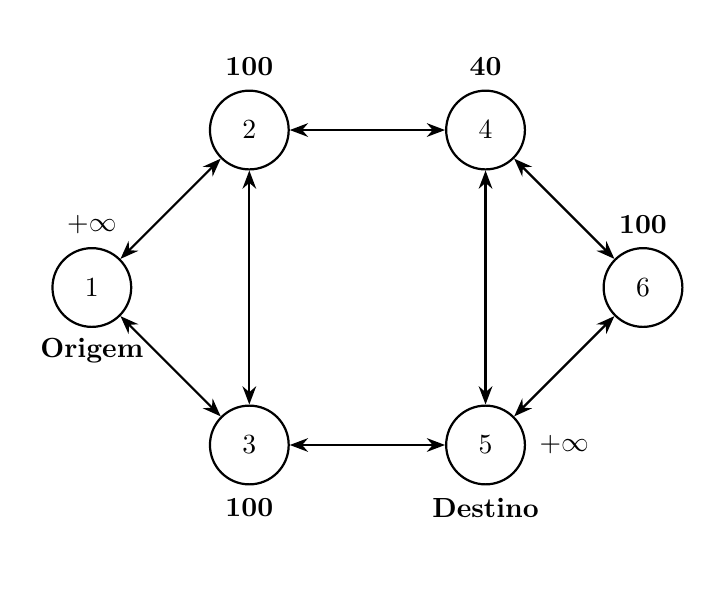
\begin{tikzpicture}[
    <->, 
    >=Stealth,
    node distance=2cm and 2.5cm,
    every node/.style={circle, draw, minimum size=1cm},
    every path/.style={thick}
]

% Nodes
\node (1) at (-2,0) {1};
\node (2) at (0,2) {2};
\node (3) at (0,-2) {3};
\node (4) at (3,2) {4};
\node (5) at (3,-2) {5};
\node (6) at (5,0) {6};

% Bidirectional edges
\draw (1) -- (2);
\draw (1) -- (3);
\draw (2) -- (3);
\draw (2) -- (4);
\draw (3) -- (5);
\draw (5) -- (6);
\draw (4) -- (6);
\draw (5) -- (4);

% Labels
\node[draw=none] at (-2, -0.8) {\textbf{Origem}};
\node[draw=none] at (3, -2.8) {\textbf{Destino}};

\node[draw=none] at (-2,0.8) {\textbf{$+\infty$}};
\node[draw=none] at (0,2.8) {\textbf{100}};
\node[draw=none] at (3,2.8) {\textbf{40}};
\node[draw=none] at (5,0.8) {\textbf{100}};
\node[draw=none] at (0,-2.8) {\textbf{100}};
\node[draw=none] at (4,-2) {\textbf{$+\infty$}};


\end{tikzpicture}
\end{center}

\end{document}